\documentclass[../DC2017114Bouma.tex]{subfiles}
\begin{document}
\graphicspath{{03_Contribution/img/}}
\renewcommand{\chaptermark}[1]{\markboth{\thechapter.\ #1}{}}
\renewcommand{\sectionmark}[1]{\markright{#1}{}}

\pagestyle{fancyreport}
\cleartooddpage
\pagestyle{fancyreport}
\chapter{Tracking for Hybrid Systems: Isolated State-and-Input-Triggered Events}\label{ch:order}
In this chapter, a control strategy is presented for trajectories of hybrid systems which, due to the introduction of perturbations, experience isolated state-and-input-triggered events. Such systems are called \textit{nonlinear state-and-input-triggered hybrid systems} (NSITHS). Isolated state-and-input-triggered events are considered, which means that the guard functions are activated separately, such that there is always flow between the events. The perturbations are assumed small enough that they can cause the state trajectory to jump at a different time than the nominal reference trajectory, but not cause the system to activate other guards or experience other events. The mismatch in event time between the nominal trajectory and state trajectory can result in \textit{peaking behavior} of the tracking error \cite{Menini2001,Biemond2013}. First, a notion of error is presented, which is used to avoid peaking behavior. After that a first-order approximation of the NSITHS is presented in the form of a \textit{linear time triggered hybrid system} (LTTHS). A proof is given in \cite{Rijnen2017}, which shows that the stability of the LTTHS can be used to asses the local stability of the original NSITHS. Consequentially, conventional stability analysis tools for LTTHS can be used to asses the local stability of te NSITHS. Finally, a short summary of the findings in this chapter is given. The work in this chapter is an extension to \cite{Rijnen2017}, where the sensitivity analysis in this chapter is suitable for input-dependent guard functions.
\nomenclature[A]{NSITHS}{Nonlinear State-and-Input-Triggered Hybrid System}%
\nomenclature[A]{LTTHS}{Linear Time Triggered Hybrid System}%

\section{State-input perturbations in trajectories with state-jumps}
This section presents \textit{reference-spreading} (RS) for ordered guard activations. First the tracking problem is presented. The perturbations introduced in the state trajectory cause the state trajectory and reference trajectory to have non-coinciding event-times. This mismatch in event-times results in peaking behavior in the tracking error, meaning that two relatively large jumps can be observed. Using reference-spreading this peaking behavior can be avoided, resulting in a tracking error where only one relatively smaller jump is observed.
\nomenclature[A]{RS}{Reference-Spreading}%

\subsection{Nonlinear state-and-input-triggered hybrid systems}
As presented in Section~\ref{sec:2hyb}, a mechanical system can be described by the hybrid system with impulsive effects framework. Such a system is a nonlinear state-and-input-triggered hybrid system. The NSITHS is now formally defined.

\begin{mydef}[NSITHS]\label{def:3nsiths}
The nonlinear state-and-input-triggered hybrid system is given by
\begin{equation}
\begin{array}{ll}
\dot{\xb}(t,j) =\fb^j(\xb(t,j),\ub(t,j),t),& \xb(t,j),\ub(t,j)\in \mathcal{C}^j\\
\xb(t,j+1) = \gb^{j+1}(\xb(t,j),\ub(t,j),t),& \xb(t,j),\ub(t,j)\in \mathcal{D}^{j+1}
\end{array}\label{eq:3hybimp}
\end{equation}
where $\fb^j$ is a nonlinear Lipschitz continuous function. $\mathcal{C}^j$ is the flow set after event $j$, and $\mathcal{D}^{j+1}$ a state-input set, where when $\xb(t,j),\ub(t,j)\in \mathcal{D}^{j+1}$ a state reinitialization is triggered according to $\xb(t,j+1) = \gb^{j+1}(\xb(t,j),\ub(t,j),t)$.
\end{mydef} 

The nominal trajectory of an NSITHS is illustrated in Figure~\ref{fig:3perturbedtraj} in red. Some minimal regularity conditions on the NSITHS are defined, which are necessary for the sensitivity analysis presented later. Formally, the following assumptions are made.

\begin{myass}[t-completeness and non-Zeno behavior of $\alphab$]
The reference trajectory $\alphab$ is defined for all $t>t_0$. Also, the reference trajectory segments $\alphab(t,j)$ have non-vanishing time-domains $I_{\alphab}^j$.\label{ass:nonzeno}
\end{myass}

Assumption~\ref{ass:nonzeno} guarantees that the number of events $N$ will only go to infinity if time $t$ goes to infinity as well. This assumption is often made in analysis using hybrid systems. It can then be guaranteed that there is non-zero time between events, if $\gb(\alphab(\tau^{j+1},j),\mub(\tau^{j+1},j),j+1)\notin \mathcal{D}^{j+1}$. The t-completeness of $\alphab$ guarantees that there is always a trajectory defined for the system to track.

Now an initial state and input perturbation $\epsilon$ is introduced, which causes the state trajectory $\xb$ to differ from the reference trajectory $\alphab$. The goal is to write a control strategy, such that the perturbed state trajectory $\xb$ will converge to the reference trajectory $\alphab$. Now an initial state-input perturbation $z_0 = \frac{\partial\xb}{\partial\epsilon}$ is introduced, where $\epsilon$ is a scalar perturbation parameter. The initial state $\alphab_0$ and input $\mub_0$ of the reference trajectory $\alphab$ is perturbed, resulting in $\xb_0(\epsilon) = \alphab_0 + \epsilon\zb_0$ and $\ub(t,j,\epsilon) = \mub(t,j) + \epsilon\vb(t,j)$. This generates a trajectory close to the reference trajectory $\alphab$, which is also dependent on the initial state and input perturbation $\epsilon$, i.e., $\xb(t,j,\epsilon)$. 

\nomenclature[V]{$\epsilon$}{The scalar perturbation parameter}%
\nomenclature[V]{$(.)_{\epsilon}$}{A variable dependent on the initial perturbation}%
\begin{figure}[h]
\centering
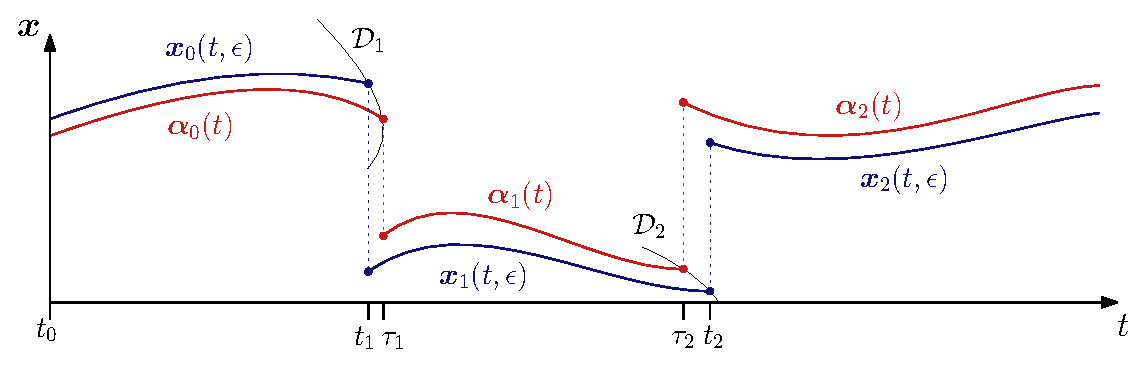
\includegraphics[width=.9\textwidth]{perturbedtraj.eps}\caption{in orange the nominal (unperturbed) and in cyan the perturbed trajectory of a hybrid system with impulsive effects. Due to the perturbation in the cyan trajectory, a mismatch between the perturbed and the nominal event times arises.} \label{fig:3perturbedtraj}
\end{figure}
For the nominal trajectory the state and input are known over the entire time-domain, meaning that the event-times are also known. For the perturbed trajectory this is not the case. Due to the uncertainty in the state and input, there is an uncertainty in the event-times as well. This uncertainty can cause a mismatch between the nominal event times $\tau^1$,$\tau^2$ and the perturbed event times $t^1$,$t^2$. Now we take a closer look at the first event, to illustrate the peaking behavior as a result of a jump mismatch. In Figure~\ref{fig:3peakerror} the state evolution $x$ of the first event is depicted besides the tracking error $||\xb-\alphab||$. Here on can clearly see that a peak arises in the tracking error when the jump times do not coincide. At $t^1$ the state trajectory jumps, while the reference trajectory does not. At $\tau^1$ the reference trajectory jumps as well. This means that in $[t^1,\tau^1]$, a post-event state trajectory is compared to a ante-event reference trajectory, resulting in a large peak in the tracking error. This is undesirable, as it will lead to large and unnecessary actuation forces.

\begin{figure}[h]
\centering
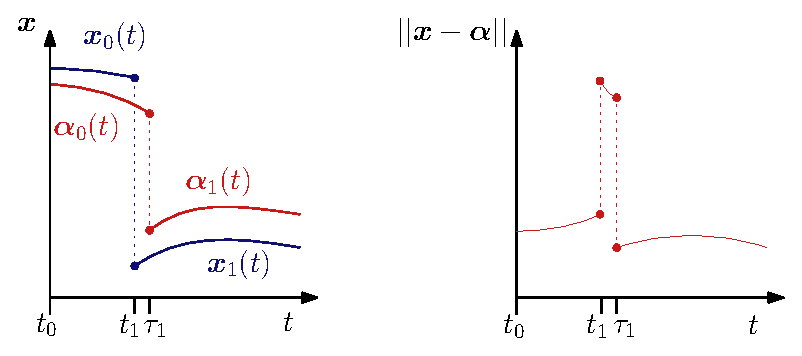
\includegraphics[width=.66\textwidth]{peakerror.eps}\caption{A closer look at the first event of the trajectory in Figure~\ref{fig:3perturbedtraj}. On the left the state-evolution $x$ is depicted and on the right the tracking error $||\xb-\alphab||$. A clear peak can be noticed in the tracking error as a result from the event-time mismatch.} \label{fig:3peakerror}
\end{figure}

In the next section a solution to the peaking behavior is presented.
\nomenclature[V]{$\Delta$}{The linearization of the perturbed event time around zero perturbation}%
\nomenclature[A]{$o(.)$}{Little-o notation}%
\nomenclature[V]{$\Gb$}{Positive homogeneous jump gain for the perturbed state direction}%
\nomenclature[V]{$\Jb$}{Positive homogeneous jump gain for the perturbed input direction}%
\nomenclature[V]{$D_i(.)$}{The derivative with respect to the $i$th term}%
\subsection{Reference-spreading}
To avoid peaking behavior in the tracking error, in \cite{Saccon2014} a novel notion of error is presented which is named reference spreading in \cite{Rijnen2016}. This control strategy uses reference trajectories which are extended beyond event-times, such that an ante-event state trajectories can always be compared to an ante-event reference trajectory and a post-event state trajectories can always be compared to a post-event reference trajectory. This is illustrated in Figure~\ref{fig:3refspread}, where the reference trajectory segments $\alphab(t,j)$ are all extended resulting in $\overline{\alphab}(t,j)$. Adopting the notation of \cite{Goebel2009}, the hybrid domain of $\alphab$ is defined by segments $I^j_{\alphab} = [\tau^j,\tau^{j+1}]$, which together form the entire domain of $\alphab$ as
\begin{align}
\dom\alphab = \bigcup^N_{j=0}I_{\alphab}^j\times\{j\}.
\end{align}
\nomenclature[P]{$I$}{Domain of a segment}%
Similarly the state segments $x(t,j)$ are defined on the domain $I^j_\xb = [t^j,t^{j+1}]$ with the entire domain defined as
\begin{align}
\dom\xb = \bigcup^N_{j=0}I_{\xb}^j\times\{j\}.
\end{align}
The domain of the extended reference trajectory segments is extended such that $I_{\xb}^j\subseteq I_{\overline{\alphab}}^j$. The set of jump times of $\alphab(t,j)$ and $\xb(t,j,\epsilon)$ are denoted as
\begin{align}
\text{eve}\ \alphab &= \bigcup_{j=1}^N \{\tau^j\}\times\{j-1\},\\
\text{eve}\ \xb &= \bigcup_{j=1}^N \{t^j\}\times\{j-1\},
\end{align}
respectively.
\begin{figure}[h]
\centering
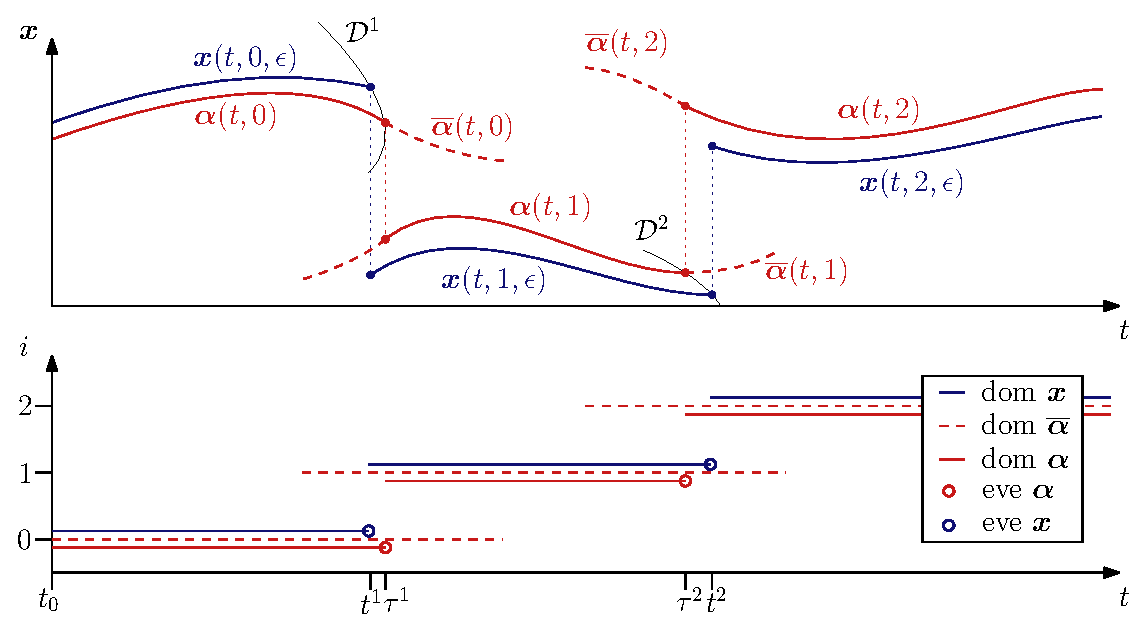
\includegraphics[width=.9\textwidth]{refspreaddom.eps}\caption{An illustration of the nominal reference trajectory (orange) and the perturbed trajectory (cyan), where the nominal reference trajectory is extended such that $\dom x\subseteq\dom \overline{\alpha}$.} \label{fig:3refspread}
\end{figure}

Now a continuity based assumption on the vector field $\fb$ is defined. This assumption uses the extended reference trajectory $\overline{\alphab}$ illustrated in Figure~\ref{fig:3refspread}.

\begin{myass}[Lipschitz continuity of $\fb$]\label{ass:lipschitz}
We assume that in a neighborhood of the reference trajectory $\alphab$, $\fb$ is Lipschitz with respect to $\xb$ uniformly in $t$ and $j$. I.e., $\exists\varepsilon_{\fb}>0$ and $\exists L$, independent of $t,j$, such that $\forall i$, $||\fb(\ab,t,j) - \fb(\bb,t,j)||<L||a-b||$, $\forall t\in (\tau^j - \varepsilon_{\fb},\tau^{j+1} + \varepsilon_{\fb})$ and $\forall \ab,\bb\in B_{\varepsilon_{\fb}}(\overline{\alphab}(t,j))$, where $B_{\varepsilon_{\fb}}(\overline{\alphab}(t,j))$ is a ball with radius $\epsilon_{\fb}$ around $\overline{\alphab}(t,j))$.
\end{myass}

In Assumption~\ref{ass:lipschitz} it is clear why the extended reference trajectory $\overline{\alphab}$ is necessary. The Lipschitz continuity condition is defined on the interval $t \in (\tau^j - \varepsilon_{\fb},\tau^{j+1} + \varepsilon_{\fb}) \supset \text{dom }\alphab$, which means that an extension of $\alphab$ is necessary to be able to define this assumption.

In the lower plot of Figure~\ref{fig:3refspread} the domains of $\xb$, $\alphab$ and $\overline{\alphab}$ are illustrated for each segment. Note that for every segment, $I_{\xb}^j\subseteq I_{\overline{\alphab}}^j$. This means that when the tracking error is defined as $||\xb-\overline{\alphab}||$, we can keep tracking the error $||\xb(t,j)-\overline{\alphab}(t,j)||$ until an event is detected. Even if the event-time $t^j>\tau^j$. When an event is detected, the error  $||\xb(t,j+1)-\overline{\alpha}(t,j+1)||$ can be tracked. Again, because $I_{\xb}^{j+1}\subseteq I_{\overline{\alphab}}^{j+1}$, this is also possible for the case where $t^j<\tau^j$. Using this notion of error leaves only one jump in the tracking error, even under the presence of event-time mismatches. More importantly, the peak in the tracking error is avoided, an ante-event state trajectory will not be compared to a post-event reference trajectory (and vice versa) anymore. In Figure~\ref{fig:3refspreaderrors} the tracking error with and without reference spreading are compared. Here it is clear that the tracking defined using reference spreading does not have the peak which the normal notion of error does have. It also jumps only once at the perturbed event-time $t_1$.
\begin{figure}[h]
\centering
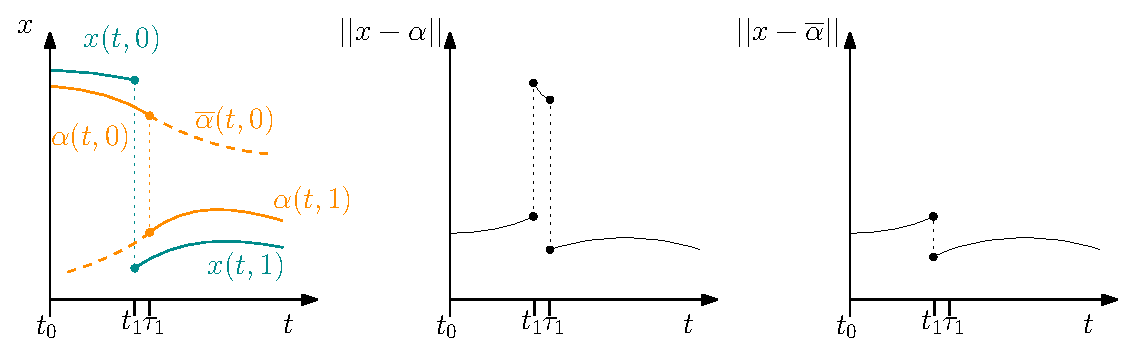
\includegraphics[width=\textwidth]{refspreaderrors.eps}\caption{A close up of the  first event of the reference trajectory, in which the peaking behavior is cleary removed by evaluating the extended reference trajectory.} \label{fig:3refspreaderrors}
\end{figure}

In the next section the error defined using reference spreading is used to make a first-order approximation of perturbed trajectories with ordered guard-activation.

\section{First-order approximation of trajectories with ordered guard-activations}\label{sec:3approx}
In \cite{Khalil1996} a sensitivity analysis is presented, where so-called sensitivity functions are used to provide first-order approximations of the effects of parameter variations on solutions. These sensitivity functions can also be used to approximate the solution under parameter variations, when the variations are close enough to zero. In the case of mechanical systems experiencing perturbations, the sensitivity equations describe the system's response the initial state-input perturbations. These perturbation dynamics can be used to formulate a first-order approximation of the perturbed state of the system. To find a first-order approximation of state reinitializations in nonsmooth trajectories, an extension to this sensitivity analysis is necessary in the form of a linearized jump gain. The linearized jump gain and the linearized perturbation dynamics together define an LTTHS, which can guarantee local asymptotic stability of the NSITHS when the LTTHS is stable \cite{Rijnen2017}. For a more thorough derivation of the analysis performed in this section, Appendix~\ref{app:Csensitivity} should be consulted. Now some assumptions are defined, which are necessary to be able to perform the sensitivity analysis.

\begin{myass}[Existence of a guard function]\label{ass:existence}
We assume that there exist constants $\varepsilon_\gamma$, and real valued guard function $\gamma(\xb,\ub,t,j)$ which is continuously differentiable with respect to $\xb$, $\ub$, and $t$, for each $j\in \{1,2,...,N\}$, such that
\begin{equation}
\begin{array}{llll}
\gamma(\xb,\ub,t,j) > 0 & &	&(\xb,\ub,t) \in B_{\varepsilon_\gamma}(\alphab(\tau,j),\mub(\tau,j),\tau)\cap \mathcal{C}^j\setminus\partial \mathcal{C}^j\\
\gamma(\xb,\ub,t,j) = 0 & &	&(\xb,\ub,t) \in B_{\varepsilon_\gamma}(\alphab(\tau,j),\mub(\tau,j),\tau)\cap \mathcal{D}^{j+1}\\
\gamma(\xb,\ub,t,j) < 0 & &	&(\xb,\ub,t) \in B_{\varepsilon_\gamma}(\alphab(\tau,j),\mub(\tau,j),\tau)\cap (\Rbb^n \times \Rbb^m \times \Rbb)\setminus \mathcal{C}^j
\end{array}
\end{equation}
where $B_{\varepsilon_{\gamma}}(\alphab(\tau,j),\tau)$ is a ball with radius $\varepsilon_{\gamma}$ around $\alphab(\tau,j)$ with $\tau = \tau^{j+1}$. $\mathcal{C}^j$ is the flow set of a trajectory after event $j$ and $\mathcal{D}^{j+1}$ is the event set which triggers event $j+1$, which is defined as $\partial \mathcal{C}^j$, where $\partial \mathcal{C}^j$ represents the boundary of flow set $\mathcal{C}^j$ (existence of a guard function).
\end{myass}

\begin{myass}[Transversal guard activations]\label{ass:transversality}
Under Assumption~\ref{ass:existence}, we assume there exists a constant $c>0$, such that
\begin{multline}
D_1\gamma(\alphab(t,j),\mub(t,j),t,j)\cdot\fb(\alphab(t,j),\mub(t,j),t,j) + D_2\gamma(\alphab(t,j),\mub(t,j),t,j)\cdot\fb(\alphab(t,j),\mub(t,j),t,j) +\\ D_3\gamma(\alphab(t,j),\mub(t,j),t,j) \leq -c,
\end{multline}
for every event time $(t,j) \in E_{\alphab}$.
\end{myass}

\begin{myremark}
The guard function time derivative of $\gamma^{\text{sl}\rightarrow\text{st}} = \sqrt{\zetab_t^T\zetab_t}$, i.e. $\dot{\gamma}^{\text{sl}\rightarrow\text{st}} = $ is undefined for $\gamma^{\text{sl}\rightarrow\text{st}}$. Therefore a Taylor expansion is used to create a first order approximation of the left limit of $\dot{\gamma}^{\text{sl}\rightarrow\text{st}}$ at $t = \tau^j$, to check whether the guard is activated transversally. More information on this can be found in Appendix~\ref{app:hybriddisc}. 
\end{myremark}

\begin{myass}[Perturbation-independent guard-event pairs]\label{ass:guardeventpair}
With the set of all participating guard functions $\gamma_{\textnormal{part}}$, we assume that there exist a constant $\varepsilon_\gamma$, and set of nominal activated guard functions $\gamma_{\textnormal{nom}}^j$, such that
\begin{align}
\gamma_{\textnormal{part}}\setminus\gamma_{\textnormal{nom}}^j > 0,\quad \forall \xb,\ub\in B_{\varepsilon_\gamma}(\alphab(\tau,j),\mub(\tau,j),\tau),
\end{align}
where $\gamma^j = \gamma(\xb,\ub,t,j)$, and $B_{\varepsilon_\gamma}(\alphab(\tau,j),\mub(\tau,j),\tau)$ is a ball with radius $\varepsilon_{\gamma}$ centered around the ante-event state and input $\alphab(\tau,j),\mub(\tau,j)$ of event $j$.
\end{myass}

Assumption~\ref{ass:existence} guarantees that the guard function exists in a ball around the nominal ante-event state. In other words, it assumes that the properties of a guard function, i.e., $\gamma>0$ in the flow set, $\gamma=0$ in the event set, and $\gamma<0$ outside of the flow set, are maintained in a ball around the nominal ante-event state $B_{\varepsilon_\gamma}(\alphab(\tau,j),\tau)$.  $\gamma(\xb,\ub,t,j) = 0$ represents the set where an event will happen, which together with Assumption~\ref{ass:transversality} guarantees that an event will happen, even under perturbations. Assumption~\ref{ass:transversality} assumes that the vector field pushes the reference trajectory out of the flow set $\mathcal{C}^j$, and that grazing incidents are avoided. The combination of the existence of a guard function in an area around the nominal ante-event state and the transversal guard activation guarantees that there exists a range of perturbations where the guard is activated as well. Assumption~\ref{ass:guardeventpair} makes sure that the perturbed trajectory will activate the same guard functions as the reference trajectory. Now an assumption of the jump maps $\gb$ is defined.

\begin{myass}[Locally differentiability of jump maps]\label{ass:jump}
We assume that for all $i \in [1,2,...,N]$ the jump map $\gb(\xb,\ub,j)$ is locally differentiable, in the sense that $D_1\gb(\xb,\ub,j)$ and $D_2\gb(\xb,\ub,j)$ exist in the ball $B_{\varepsilon_{\gamma}}(\alphab(\tau,j),\tau)$, where $B_{\varepsilon_{\gamma}}$ is the ball in which $\gamma$ exist and $\tau = \tau^{j+1}$.
\end{myass}

The differentiability of the jump map is necessary to make a first-order approximation of the perturbed state trajectory. This is explained in more detail in the next section.

\subsection{Sensitivity analysis}
The sensitivity analysis for the continuous segments of a perturbed trajectory, gives a set of equations which describe the systems reaction to an initial state-input perturbation. The perturbed state is defined as
\begin{align}
\xb(t,j,\epsilon) = \xb(t_0,j,\epsilon) + \int_{t_0}^{t}\fb^j(\xb(s,j,\epsilon),\ub(s,j,\epsilon),s)ds,\label{eq:3xpert}
\end{align}
with the input chosen as $\ub(t,j,\epsilon) = \overline{\mub} - \Kb\left(\xb(t,j,\epsilon)-\alphab(t,j)\right)$, where $\overline{\mub}$ is a feedforward term that generates the reference trajectory $\alphab$ and $\Kb\left(\xb(t,j,\epsilon)-\alphab(t,j)\right)$ is a feedback term to achieve tracking of the reference. To find a first-order approximation of the perturbed state, the perturbed state direction $\zb(t)$ and the perturbed input direction $\vb(t)$ are defined as
\begin{align}
\zb(t,j) = \left.\frac{\partial\xb(t,j,\epsilon)}{\partial\epsilon}\right|_{\epsilon=0},\text{ and } \vb(t,j) = \left.\frac{\partial\ub(t,j,\epsilon)}{\partial\epsilon}\right|_{\epsilon=0}=-\Kb(t)\zb(t).
\end{align}
Then the sensitivity analysis in \cite{Khalil1996} gives a first-order approximation of the state based on a Taylor series of $\xb^j(t,\epsilon)$ with respect to $\epsilon$ as
\begin{align}
\xb(t,j,\epsilon) &= \xb(t,j,0) + \epsilon\left.\frac{\partial\xb(t,j,\epsilon)}{\partial\epsilon}\right|_{\epsilon=0} + o(\epsilon),\label{eq:3taylor}\\
&= \alphab(t,j) + \epsilon\zb(t,j) + o(\epsilon),
\end{align}
with $o(\epsilon)$ indicating the little-o notation of $\epsilon$ which represents higher order terms. To find a first order approximation of the $\dot{\xb}(t,j,\epsilon)$, an expression for $\dot{\zb}(t,j)$ should be found. By first taking the partial derivative with respect to $\epsilon$ and then with respect to $t$ of $\eqref{eq:3xpert}$, the perturbation dynamics are found to be
\begin{align}
\dot{\zb}(t,j) = \Ab(t,j)\zb(t,j) +\Bb(t,j)\vb(t,j),
\end{align}
with
\begin{align}
\Ab(t,j) &= D_1\fb(\alphab(t,j),\mub(t,j),t,j),\\
\Bb(t,j) &= D_2\fb(\alphab(t,j),\mub(t,j),t,j),
\end{align}
where $D_a$ is defined as the partial derivative of the function that follows with respect to the $a^{\text{th}}$ argument of that function evaluated at $\epsilon = 0$. The first order approximation of the perturbed state dynamics in continuous time is then defined as
\begin{align}
\dot{\xb}(t,j,\epsilon) \approx \dot{\alphab}(t,j) + \epsilon\dot{\zb}(t,j),
\end{align}
where $\dot{\alphab}(t,j)$ is known from the tracked reference trajectory and $\dot{\zb}(t,j)$ is known from the sensitivity analysis performed on the system. Now the first-order approximation is defined for the continuous segments of a trajectory. What remains is that the state reinitializations should be linearized as well. The reinitialization of the nominal trajectory is described by
\begin{align}
\alphab(\tau^j,j) = \gb(\alphab(\tau^j,j-1),\mub(\tau^j,j-1),\tau^j,j),\label{eq:3g}
\end{align}
and the reinitialization of the perturbed state is described by (due to Assumption~\ref{ass:lipschitz}, \ref{ass:guardeventpair}, and \ref{ass:jump})
\begin{align}
\xb(t^{j},j,\epsilon) = \gb(\xb(t^{j},j-1,\epsilon),\ub(t^{j},j-1,\epsilon),t^{j},j).
\end{align}
Similar to the Taylor expansion used in \eqref{eq:3taylor}, the state and input of the next segment evaluated at the perturbed event time $t^{j}$ can be expanded to
\begin{align}
\xb(t^{j},j,\epsilon) &= \overline{\alphab}(t^{j},j) + \epsilon\zb(t^{j},j) + o(\epsilon),\label{eq:3xexpand}\\
\ub(t^{j},j,\epsilon) &= \overline{\mub}(t^{j},j) + \epsilon\vb(t^{j},j) + o(\epsilon).\label{eq:3uexpand}
\end{align}
The same can be done for $\alphab(t^{j},j)$, $\mub(t^{j},j)$, $\zb(t^{j},j)$, and $\vb(t^{j},j)$, which when substituted into \eqref{eq:3xexpand} and \eqref{eq:3uexpand} result in
\begin{align}
\xb(t^{j},j,\epsilon) &= \alphab(\tau^j,j) + \epsilon\dot{\alphab}(\tau^j,j)\Delta + \epsilon\zb(\tau^j,j) + o(\epsilon),\label{eq:3xexpand2}\\
\ub(t^{j},j,\epsilon) &= \mub(\tau^j,j) + \epsilon\dot{\mub}(\tau^j,j)\Delta + \epsilon\vb(\tau^j,j) + o(\epsilon),\label{eq:3uexpand2}
\end{align}
with
\begin{align}
\Delta^{j} = \left.\frac{\partial t^{j}}{\partial\epsilon}\right|_{\epsilon=0}.\label{eq:3Delta}
\end{align}
To find $\Delta^{j}$ we evaluate the ante-event guard function
\begin{align}
\gamma(\xb(t^{j},j-1,\epsilon),\ub(t^{j},j-1,\epsilon),t^{j},j) = 0,\label{eq:3gamma}
\end{align}
where $\gamma$ is evaluated at the left limit of event $j$. Due to Assumptions~\ref{ass:lipschitz}, \ref{ass:existence}, and \ref{ass:transversality} it is guaranteed that the solution of \eqref{eq:3gamma} is close to the nominal solution. Note that $\gamma$ is dependent on the input $\ub$, whereas in \cite{Chen2018a} the sensitivity analysis is performed for guard functions which solely depend on state $\xb$ and time $t$. From \eqref{eq:3gamma} the expression for $\Delta^{j}$ is found to be
\begin{align}
\Delta^{j} = -\frac{D_1\gamma^{-}\cdot\zb^- + D_2\gamma^{-}\cdot\vb^-}{\dot{\gamma}^{-}},\label{eq}
\end{align}
with
\begin{align}
\gamma^- &= \gamma(\alphab(\tau^j,j-1),\mub(\tau^j,j-1),\tau^j,j),\\
\dot{\gamma}^- &= D_1\gamma^-\cdot\dot{\alphab}(\tau^j,j-1) + D_2\gamma^-\cdot\dot{\mub}(\tau^j,j-1) + D_3\gamma^-,\\
\zb^- &= \zb(\tau^j,j-1),\\
\vb^- &= \vb(\tau^j,j-1),
\end{align}
where the $-$ superscript indicates a left limit of event $j$. Now \eqref{eq:3g} is expanded and substituted  into \eqref{eq:3xexpand2} to find
\begin{equation}
\zb^+ = D_1\gb^-\cdot\left(\zb^- + \dot{\alphab}^-\Delta^j\right) + D_2\gb^-\cdot\left(\vb^- + \dot{\mub}^-\Delta^j\right) + D_3\gb^-\cdot\Delta^j - \dot{\alphab}^+\Delta^j,
\end{equation}
with
\begin{align}
\gb^- &= \gb(\alphab(\tau^j,j-1),\mub(\tau^j,j-1),\tau^j,j),\\
\zb^+ &= \zb(\tau^j,j),\\
\alphab^- &= \alphab(\tau^j,j-1),\\
\alphab^+ &= \alphab(\tau^j,j),\\
\mub^- &= \mub(\tau^j,j-1).
\end{align}
Here the $+$ superscript indicates the right limit of event $j$. This can finally be rewritten to
\begin{align}
\zb^+ = \Lb(\tau^j,j)\begin{bmatrix}
\zb^- \\ \vb^-
\end{bmatrix},
\end{align}
with 
\begin{align}
\Lb(\tau^j,j) &= \begin{bmatrix}
\Gb(\tau^j,j) & \Jb(\tau^j,j)
\end{bmatrix},\\
\Gb(\tau^j,j) & = D_1\gb^- - \left(\dot{\gb}^- - \fb^+\right)\frac{D_1\gamma^-}{\dot{\gamma}^-},\\
\Jb(\tau^j,j) & = D_2\gb^- - \left(\dot{\gb}^- - \fb^+\right)\frac{D_2\gamma^-}{\dot{\gamma}^-},
\end{align}
where
\begin{align}
\fb^- &= \fb(\alphab(\tau^j,j-1),\mub(\tau^j,j-1),\tau^j,j-1),\\
\fb^+ &= \fb(\alphab(\tau^j,j),\mub(\tau^j,j),\tau^j,j),\\
\dot{\gb}^- &= D_1\gb^-\cdot \fb^- + D_2\gb^-\cdot \dot{\mub}^- + D_3\gb^-.
\end{align}
Due to Assumptions~\ref{ass:existence} and \ref{ass:jump}, the derivatives of the jump map $\gb$ and the guard function $\gamma$ exist locally. Therefore, the linearized jump gains $\Gb$ and $\Lb$ are defined locally as well.

\subsection{Linear time triggered hybrid system}
Now the sensitivity analysis performed in previous section is used to define the LTTHS associated to reference trajectory $\alphab$ and the NSITHS defined in Definition~\ref{def:3nsiths}. The LTTHS converts the state-triggered behavior of the NSITHS to a time-triggered behavior using a first order approximation of the state jumps. Where the jump times for NSITHS are unknown for perturbed trajectories, the LTTHS jumps at the same event-times as the nominal trajectory $\alphab$. In \cite{Rijnen2017} a proof is given that stability of the LTTHS implies local asymptotic stability of the NSITHS. Since the stability assessment of LTTHS is well established in literature, the LTTHS can be used to conveniently assess the local asymptotic stability of the NSITHS. Now the LTTHS is formally defined.
\begin{mydef}[LTTHS]\label{def:3ltths}
The linear time-triggered hybrid system associated with the reference trajectory $\alpha$ and the NSITHS is given by
\begin{align}
\dot{\zb}(t,j) &= \Ab(t,j)\zb(t,j) + \Bb(t,j)\vb(t,j) &(t,j)\in \dom\ \alphab\\
\zb^+ &= \Gb(t,j)\zb^- + \Jb(t,j)\vb^- &(t,j)\in \eve\ \alphab
\end{align}
with initial condition $\zb(t_0,0)=z_0$, $\zb^+ = \zb(\tau^j,j)$, $\zb^- = \zb(\tau^j,j-1)$,
\begin{align}
\Ab(t,j) &= D_1\fb(\alphab(t,j),\mub(t,j),t,j)\\
\Bb(t,j) &= D_2\fb(\alphab(t,j),\mub(t,j),t,j)\\
\Gb(t,j) & = D_1\gb^- - \left(\dot{\gb}^- - \fb^+\right)\frac{D_1\gamma^-}{\dot{\gamma}^-},\\
\Jb(t,j) & = D_2\gb^- - \left(\dot{\gb}^- - \fb^+\right)\frac{D_2\gamma^-}{\dot{\gamma}^-},
\end{align}
and
\begin{align}
\fb^- &= \fb(\alphab(\tau^j,j-1),\mub(\tau^j,j-1),\tau^j,j-1),\\
\fb^+ &= \fb(\alphab(\tau^j,j),\mub(\tau^j,j),\tau^j,j),\\
\gb^- &= \gb(\alphab(\tau^j,j-1),\mub(\tau^j,j-1),\tau^j,j),\\
\dot{\gb}^- &= D_1\gb^-\cdot \fb^- + D_2\gb^-\cdot \dot{\mub}^- + D_3\gb^-,\\
\gamma^- &= \gamma(\alphab(\tau^j,j-1),\mub(\tau^j,j-1),\tau^j,j),\\
\dot{\gamma}^- &= D_1\gamma^-\cdot\dot{\alphab}(\tau^j,j-1) + D_2\gamma^-\cdot\dot{\mub}(\tau^j,j-1) + D_3\gamma^-.
\end{align}
\end{mydef}
The LTTHS defined in Definition~\ref{def:3ltths} gives a first order approximation of a perturbed trajectory of the NSITHS. With a nominal trajectory $\alphab$ with input $\mub$, the perturbed trajectory $\xb(t,j,\epsilon)$ is the trajectory generated by initial condition $\xb_0(\epsilon) = \alphab_0 + \epsilon\zb_0$ and input $\ub(t,j,\epsilon) = \mub(t,j) + \epsilon\vb(t,j)$. The first order approximation is then defined as $\xb(t,j,\epsilon) \approx \alphab(t,j) + \epsilon\zb(t,j)$, with $\zb$ defined by the LTTHS. Note that the approximation jumps at the same time instants as the nominal trajectory, with $(t,j) \in \eve\ \alphab$. This results in a trajectory which is generally infeasible around the jump times. However, due to the short timescales of the events, we are more interested in finding a good approximation of the continuous segments between the events, which is what the LTTHS achieves. Since $\zb = \frac{\partial\xb}{\partial\epsilon}$, an LTTHS with an equilibrium at $\zb = 0$ implies tracking of $\alphab$. Therefore, the feedback gains for the input $\vb(t,j) = -\Kb(t,j)\zb(t,j)$ should be chosen in such a way that this is achieved. Straightforward stability analysis tools for LTTHS are available in the literature, about which more can be read in Appendix~\ref{app:LTTHSstab}. Finally, one should realize that the term $\vb^-$ is not an input that can be freely chosen. $\vb^-$ is directly related to $\vb(t,j)$, as it is a result of the feedback law implemented during the continuous segment before the event.

\begin{figure}[h]
\centering
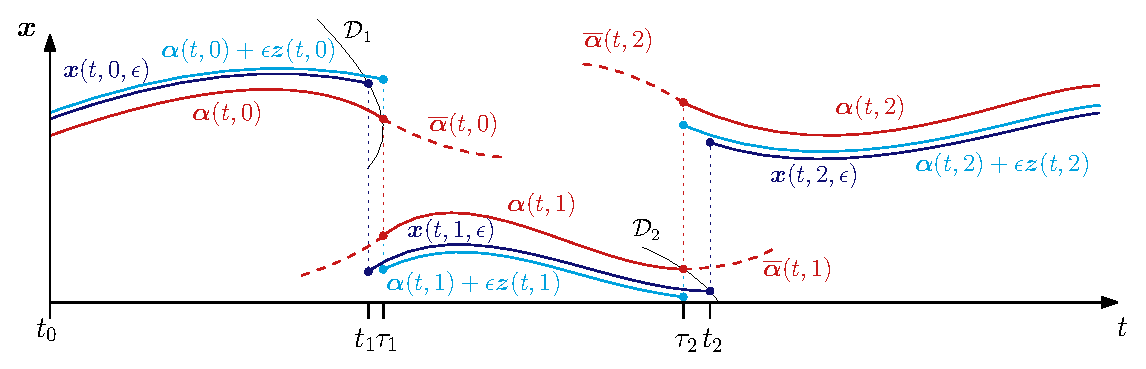
\includegraphics[width=.95\textwidth]{refspreadapprox.eps}\caption{The first order approximation $\alphab + \epsilon\zb$ (cyan) generated by the LTTHS is illustrated besides the perturbed trajectory $\xb$ (blue) and the nominal trajectory $\alphab$ (red). Note that the event times of the approximation are the same as those of the nominal trajectory.} \label{fig:3refspreadapprox}
\end{figure}


\section{Summary}
In this chapter a control strategy is presented to achieve tracking of trajectories with single guard activations for nonlinear state input triggered hybrid systems. The NSITHS is formally defined, which is a framework suitable for the dynamics defined in Chapter~\ref{ch:model}. An initial state and input perturbation is introduced into this system, generating perturbed trajectories of which the perturbed event times differ from the nominal event times, and are not known beforehand. This mismatch in event time leads to a behavior called peaking, generating undesirable actuation forces. Reference spreading is then presented to avoid peaking behavior, which leads to less and smaller jumps in the tracking error. Then, under certain assumptions, a sensitivity analysis is performed. The sensitivity analysis leads to a LTTHS describing the tracking error dynamics, which is used to generate a first order approximation of the perturbed state. This LTTHS can be evaluated using conventional stability analysis tools, considering that stability of the LTTHS implies tracking of the nominal reference trajectory.
%% new chapter %%
\cleartooddpage
\chapter{Tracking for Hybrid Systems: Simultaneous State-and-Input-Triggered Events}\label{ch:simult}
In this chapter the control strategy presented in Chapter~\ref{ch:order} is extended to be suitable for trajectories with simultaneous guard activations. Simultaneous guard activations are activations where a trajectory triggers two guard functions at the same time-instant. Take for example a box with two contact points, where the contact points make contact with a surface at the same time. When perturbations are introduced in these trajectories, the simultaneity of the event can get lost. Also, the order of activations can change depending on the perturbation. The box can first make contact with one contact point and then with the other, or the other way around. This complicates the definition of the first-order approximation. In this chapter, a novel notation from \cite{Rijnen2018} is presented to describe trajectories with simultaneous guard functions. Reference spreading is applied to trajectories with simultaneous events, which is used as basis to define a positive homogeneous jump gain which approximates the jump behavior of the perturbed trajectory. The positive homogeneous jump gain defines the \textit{positive homogeneous time-triggered hybrid system} (PTHHS), whose stability implies local asymptotic stability of the NSITHS. This chapter extends the work presented in \cite{Rijnen2018} to being suitable for input-dependent guard functions, and therefore mechanical systems experiencing dry friction and releasing motions.

\section{Simultaneous guard-activation}
To be able to perform the sensitivity analysis presented in Chapter~\ref{ch:order} for trajectories with simultaneous guard activations, some adjustments need to be made to the notation. In this section a new notation, introduced in \cite{Rijnen2018}, is presented, namely: the event character, micro- and macro-events, multiscale hybrid time, guard function index, mode descriptor, phantom segments, and historical notation. After this, reference spreading for simultaneous guard-activations is discussed.

\subsection{Adopted notation}
In a simultaneous event, more than one guard function is activated in one event. In Figure~\ref{fig:4simulexample} an example of a simultaneous activation is illustrated. The ante-event reference trajectory, $\alphab(t,0)$, activates two guard functions, $\gamma^1$ and $\gamma^2$. The number of guard functions that are activated in a single nominal event is called the \textit{event character}. In the example in Figure~\ref{fig:4simulexample}, the event character $c = 2$.

\begin{figure}[h]
\centering
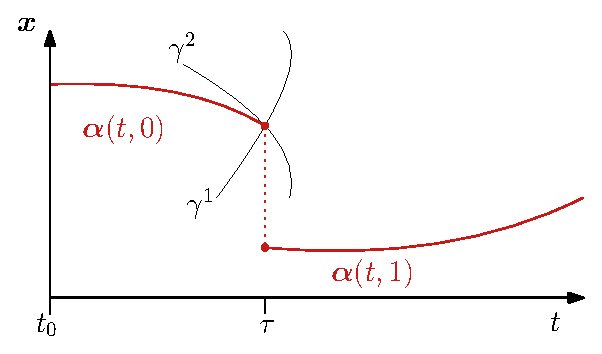
\includegraphics[width=.45\textwidth]{simulexample.eps}\caption{An illustration of a trajectory going through a simultaneous event. At $t=\tau$, the trajectory activates two guard functions, $\gamma^1$ and $\gamma^2$.} \label{fig:4simulexample}
\end{figure}

When perturbations are introduced in an event with simultaneous activations, the number of events the system goes through can change. Instead of a simultaneous activation of a $c$ guards, the guards can be activated in rapid succession. These events that are the result of loss of simultaneity are called \textit{micro-events}, where several micro-events form one \textit{macro event}. Micro-events will generate extra segments in the state trajectory in comparison to the reference trajectory. To keep track of these segments, \textit{multiscale hybrid time} is introduced. Multiscale hybrid time is denoted by $(t,i,k)$, where $t$ is regular time, $i$ the macro-event counter, and $k$ the micro-event counter. The micro-event counter $k$ is incremented everytime an event occurs, except when a macro event is completed by reaching the nominal post-event mode. The micro-event counter $k$ then resets to $0$, and the macro-event counter $i$ is incremented. One can now write $\xb(t,i,k)$ to make a distinction between all the segments that generated as a result of loss of simultaneity. Multiscale hybrid is directly related to the regular hybrid time, according to
\begin{align}
j(i,k) = k + \sum_{I=0}^{i}l_I,
\end{align}
where $l_I$ is the number of micro-events in macro-event $I$. The perturbed event times of micro-events are denoted by $t_k^i$, which is event time of the $k^{\text{th}}$ micro-event of macro-event $i$. A guard function index $\eta$ is introduced to identify the several guard functions that are involved with a macro-event. The guard functions of macro-event $i$ are given by $\gamma_{\eta}^i$, with
\begin{align}
\eta = 2^{\nu},\quad\text{with }\nu\in\{0,1,...,c^i\}.
\end{align}
$\eta$ is written in the binary numeral system for a more intuitive notation of the different guard functions. The modes that the system is in, is indicated using the \textit{mode descriptor} $s_k^i$. The mode descriptor $s_k^i$ is associated to event $i$, similar to $\tau^i$. It should no be confused with the hybrid time $i$, which defines a segment rather than a point. The micro-segments around contact point $i$ can be described using
\begin{align}
\ls^{s_k^i}\xb(t) = \xb(t,i-1,k),
\end{align}
with $s_k^i$ the mode of the $k^{\text{th}}$ micro-event associated to macro-event $i$. Similar to $\eta$, the mode descriptor is written in the binary numeral system. For example, when the event character $c^i = 2$, the guard functions that are involved with that macro event are $\gamma^i_{10}$ and $\gamma^i_{01}$. The system begins in mode $s^i_0 = 00$, where $\gamma^i_{10},\gamma^i_{01}>0$. When the state activates one of the guard functions, for example $\gamma^i_{01}=0$, the next mode becomes $s^i_1 = 01$. When the other guard function is activated as well, $\gamma^i_{10} = 0$, the system completes its macro-event with $s^i_2 = 0$. This is illustrated in Figure~\ref{fig:4simulpert}. \textbf{MAKE EXAMPLE MORE CLEAR WITH BLOCK}

\begin{figure}[h]
\centering
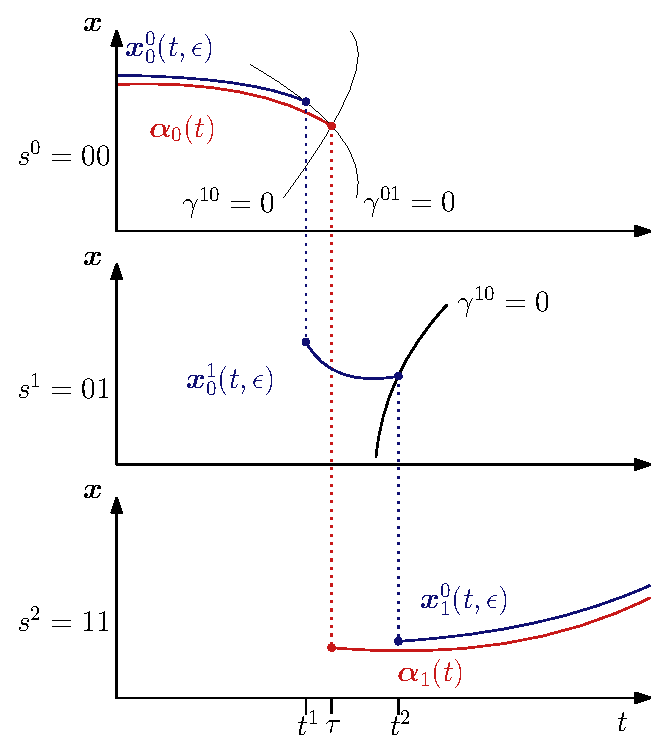
\includegraphics[width=.52\textwidth]{simulpert.eps}\caption{A reference trajectory going through a simultaneous event and a state trajectory experiencing loss of simultaneity are illustrated in this figure. Where the reference trajectory activates $\gamma^{10}$ and $\gamma^{01}$ simultaneously, the state trajectory first activates $\gamma^{01}$ at $t=t_1^1$, flows for $t\in [t_1^1,t_2^2]$, and then activates $\gamma^{10}$ at $t=t_2^1$.}\label{fig:4simulpert}
\end{figure}

Depending on the perturbation, several mode sequences can achieve the expected nominal end mode when simultaneity is lost. The different mode sequences can generate a different post-event state, since the differential equation that describes the micro-segments in between the micro-events change with their mode. Therefore, it is useful to be able to indicate an entire mode sequence with one variable. We call this notation the \textit{historical notation}. We define the growing sequence $S_k^i$ as 
\begin{align}
S_k^i = s_k^i\leftarrow s_{k-1}^i\leftarrow ... \leftarrow s_0^i,
\end{align}
where $s_0^i = 00...0$ with length $c^i$. A growing mode sequence is a sequence of micro-events, where at eacht micro-event another guard function is activated and no guard functions deactivated. We can now define $^{S_k^i}\xb(t)$ as $^{s_k^i}\xb(t)$ that is a result of the growing sequence $S_k^i$. The jump maps that are applied during such a sequence are given by
\begin{align}
\ls^{p}\xb = \ls^{p\leftarrow a}\gb(\ls^{a}\xb,\ls^{a}\ub,t),
\end{align}
where $p$ represents the post-event mode descriptor, and $a$ the ante-event mode descriptor. For example, the state jump from $s^i_k$ to $s^i_{k+1}$ is given by $\ls^{s^i_{k+1}}\xb = \ls^{s^i_{k+1}\leftarrow s^i_k}\gb(\ls^{s^i_k}\xb,\ls^{s^i_k}\ub,t)$. When the considered macro-event is known form context, the macro-counter $i$ can be dropped to simplify the notation. Growing sequences with a particular order of events are now given by
\begin{align}
\ls^{\nu_k \nu_{k-1}...\nu_{1}}S_k = s_k \leftarrow s_{k-1} \leftarrow ... \leftarrow s_0,
\end{align}
where all mode descriptor entries are defined as $s_{\kappa} = s_{\kappa-1} + \eta_{\kappa}$, with $\eta_{\kappa} = 2^{\nu_{\kappa}-1}$ and $\kappa = \{1,2,...,k\}$. For a simultaneous activation during a micro-event, the participating guard functions are placed withing brackets. For example, for a character-4 ($c^i = 4$) growing sequence, we write 
\begin{align}
\ls^{23(14)}S_3 = 1111 \leftarrow 1101 \leftarrow 1001 \leftarrow 0000.
\end{align}
Now that the notation for trajectories with simultaneous guard activations is in place, the analysis of these systems can be discussed.
\nomenclature[C]{$\kappa$}{Historical notation counter}%
\subsection{Reference-spreading for simultaneous events}
For trajectories with simultaneous activations, the perturbed state can experience more events than the reference trajectory. The perturbed state will enter micro-modes and micro-segments, which are undefined in the reference trajectory. To be able to define a physically realistic comparison between the reference trajectory and the state trajectory, the reference trajectory needs to be adjusted accordingly. This is done in the form of \textit{nominal phantom modes} and \textit{nominal phantom segments}. Phantom modes are modes defined in the reference trajectory, that do not physically exist. Before these phantom modes are defined, an assumption needs to be made on the jump maps. This assumption is now formally defined.
\begin{myass}[Associativity of jump maps]\label{ass:associativity}
We assume that the jump map $\ls^{p\leftarrow a}\gb(\ls^{a}\xb,\ls^{a}\ub,t)$ is associative, meaning that taking an arbitrary growing sequence $s_k\leftarrow s_{k-1} \leftarrow ... \leftarrow s_0$, where $p = s_k$ and $a = s_0$, one can say
\begin{align}
\ls^{p}\xb = \left(\ls^{p\leftarrow s_{k-1}}\gb \circ \ls^{s_{k-1} \leftarrow s_{k-2}}\gb \circ \cdots \circ \ls^{s_1 \leftarrow a}\gb \right).
\end{align}
Intuitively, this means that the simultaneous jump gain from $a$ to $p$ can be described with a sequence of jump gains evaluated on the same time instant.
\end{myass}
Using Assumption~\ref{ass:associativity}, the phantom modes can be defined. All micro-modes, which the state can enter as a result of loss of simultaneity, are defined in the nominal trajectory. These modes are called the phantom modes in the nominal trajectory. The initial states associated to these modes are found by applying the corresponding jump maps $\ls^{p\leftarrow a}\gb$ to the nominal ante-event state,
\begin{align}
\ls^{s^i_1}\alphab =&\ \ls^{s^i_1\leftarrow s^i_0}\gb(\ls^{s^i_0}\alphab,\ls^{s^i_0}\mub,\tau^i)\nonumber\\
&\vdots\label{eq:4phantomini}\\
\ls^{s^i_{k}}\alphab =&\ \ls^{s^i_k\leftarrow s^i_{k-1}}\gb(\ls^{s^i_{k-1}}\alphab,\ls^{s^i_{k-1}}\mub,\tau^i),\nonumber
\end{align}
resulting in a reference trajectory that goes through the same modes as the state trajectory. The feedforward term that defines the phantom modes can be chosen from two options. We define \textit{withdrawing phantom modes} and \textit{pushing phantom modes}, which are defined by the feedforwards
\begin{equation}
\ls^{S_k^i}_{\nearrow}\overline{\mub}(t) := \left\lbrace\begin{array}{ll}
\overline{\mub}(t,i-1), & k = 0\\
\overline{\mub}(t,i), & k \neq 0
\end{array},\right.
\end{equation}
and
\begin{equation}
\ls^{S_k^i}_{\searrow}\overline{\mub}(t) := \left\lbrace\begin{array}{ll}
\overline{\mub}(t,i-1), & k \neq l_i\\
\overline{\mub}(t,i), & k = l_i
\end{array},\right.\label{eq:4phantominp}
\end{equation}
\nomenclature[P]{$l_i$}{Number micro-events in macro-event $i$}%
where $\nearrow$ indicates a withdrawing feedforward and $\searrow$ indicates a pushing feedforward, and $l_i$ the number of micro-events associated with macro-event $i$. For each event it should be defined whether a withdrawing or pushing phantom mode is used. 

Since the events of the state trajectory happen at different time-instant than the events in the reference trajectory, the phantom modes should be extended similarly as in Section~\ref{ch:order}. 
Using the initial states $\ls^{S^i_{k}}\alphab$ defined in \eqref{eq:4phantomini} and inputs $\ls^{S_k^i}\overline{\mub}$ defined in \eqref{eq:4phantominp}, the vector field $\ls^{s_k^i}\fb$ can be integrated forward and backward to find the (pushing or withdrawing) phantom segments corresponding to the phantom modes. These phantom modes and segments are illustrated in Figure~\ref{fig:4simulmicro}, where $\overline{\alphab}(t,0,1),\overline{\alphab}(t,1,1),\overline{\alphab}(t,1,2)$ are examples of phantom segments.
\begin{figure}[h]
\centering
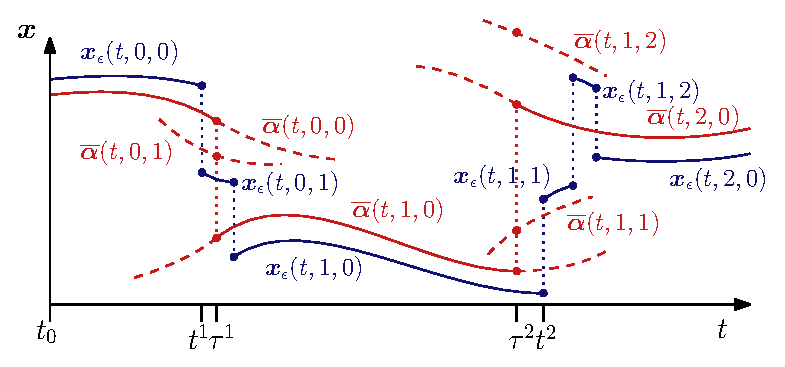
\includegraphics[width=.8\textwidth]{simulmicro.eps}\caption{The state evolution of the reference trajectory and state trajectory. Phantom segments are added to the reference trajectory, to which the micro-segments of the state trajectory can be compared.}\label{fig:4simulmicro}
\end{figure}

\nomenclature[C]{$k$}{The micro-event counter}%
\nomenclature[C]{$j$}{The classic hybrid-time event counter}%
\nomenclature[P]{$c_i$}{The event-character of macro-event $i$}%
\nomenclature[P]{$l_i$}{The amount of simultaneous activations of macro-event $i$}%
\nomenclature[V]{$s^k_i$}{The event-mode descriptor of macro-event $i$ and micro-event $k$}%
\nomenclature[V]{$S^k_i$}{The historical notation of macro-event $i$ from micro-event $0$ up to $k$}%
\nomenclature[V]{$\eta$}{A guard function identifier}%
\nomenclature[V]{$\chi$}{The set of guard function identifiers of guards that can be activated}%
\nomenclature[V]{$t_i^k$}{The perturbed event time of macro-event $i$ and micro-event $k$}%

\section{First-order approximation for trajectories with simultaneous guard-activation}
Now the sensitivity analysis for a trajectory with simultaneous events is presented. Similar to the sensitivity analysis for trajectories with isolated events, the continuous segments of the state can be approximated using
\begin{align}
\xb(t,i,\epsilon) = \alphab(t,i) + \epsilon\zb(t,i) + o(\epsilon),
\end{align}
where $\zb(t,i)$ is defined by
\begin{align}
\dot{\zb}(t,i) = \Ab(t,i)\zb(t,i) +\Bb(t,i)\vb(t,i),
\end{align}
with
\begin{align}
\Ab(t,i) &= D_1\fb(\alphab(t,i),\mub(t,i),t,i),\\
\Bb(t,i) &= D_2\fb(\alphab(t,i),\mub(t,i),t,i).
\end{align}
Now we derive a first order approximation of the jump map of a simultaneous event with character $c^i = 2$. A more thorough description of this derivation can be found in Appendix~\ref{app:multjumps}. In this Chapter, the macro-counter $i$ is left out of the derivation as it is redundant. The jump map that describes this jump is given by
\begin{align}
\ls^{s^{k+1}}\xb_\epsilon(t^{k+1}) = \ls^{s^{k+1}\leftarrow s^k}\gb(\ls^{s^{k}}\xb_\epsilon(t^{k+1}),\ls^{s^{k}}\ub_\epsilon(t^{k+1}),t^{k+1}),\label{eq:4xe012}
\end{align}
with
\begin{align}
\ls^{s^{k}}\xb_\epsilon(t^{k+1}) = \int_{t^{k}}^{t^{k+1}}\left[\ls^{s^{k}}\fb\left(\ls^{s^{k}}\xb_\epsilon(t),\ls^{s^{k}}\ub_\epsilon(t),t\right)\right]dt + \ls^{s^{k}\leftarrow s^{k-1}}\gb(\ls^{s^{k-1}}\xb_\epsilon(t^{k}),\ls^{s^{k-1}}\ub_\epsilon(t^{k}),t^{k}).\label{eq:4xe01}
\end{align}
Here the subscript $(.)_\epsilon$ indicates that the variable is dependent on $\epsilon$, the left superscript $\ls^{s^k}(.)$ indicates that the variable is in micro-segment $k$, and $t^k$ represents the event-time of micro-event $k$. Now we expand the right-hand side of \eqref{eq:4xe012} with respect to $\epsilon$, to find
\begin{align}
\ls^{s^{k+1}}\xb_\epsilon(t^{k+1}) = \ls^{s^{k+1}}\alphab(\tau) + \epsilon\left.\frac{\partial}{\partial\epsilon}\ls^{s^{k+1}\leftarrow s^k}\gb\right|_{\epsilon=0} + o(\epsilon),\label{eq:4xe012exp}
\end{align}
where
\begin{multline}
\left.\frac{\partial}{\partial\epsilon}\ls^{s^{k+1}\leftarrow s^k}\gb\right|_{\epsilon=0} = D_1\ls^{s^{k+1}}\gb\cdot\left(\ls^{s^{k}}\fb(\Delta^{k+1}-\Delta^{k}) + D_1\ls^{s^{k}}\gb\cdot\left(\ls^{s^{k-1}}\zb+\ls^{s^{k-1}}\fb\Delta^{k}\right)\right. \\ \left.+ D_2\ls^{s^{k}}\gb\cdot\left(\ls^{s^{k-1}}\vb+\ls^{s^{k-1}}\dot{\mub}\Delta^{k}\right) + D_3\ls^{s^{k}}\gb\cdot\Delta^{k}\right)+D_3\ls^{s^{k+1}}\gb\cdot\Delta^{k+1}. \label{eq:4dg1de}
\end{multline}

\begin{mydef}[Positive homogeneity]
Suppose that $\fb(\xb,\ub,t)$ is a continuously differentiable function. The function $\fb$ is called positive homogeneous to the degree $k$, if 
\begin{align}
\fb(a\xb,a\ub,t) = a^k\fb(\xb,\ub,t),
\end{align}
for all constants $a>0$.
\end{mydef}

\begin{myass}[Growing mode sequences]
We assume that all considered mode sequences are growing, meaning that at each micro-event, one or more guard functions become active, without changing the status of any other guard-function. In other words, considering one macro-event, we assume that $s^0<s^1<...s^l$, where $s^0= 00...0$ and $s^l = 11...1$, and $l$ is the number of micro-events in the considered macro-event.
\end{myass}

\begin{itemize}
\item Positive homogeneous jump gain derivation
\item Effect of $\vb = 0$ on pos hom jump gain
\item PTTHS (Positive homogeneous time-triggered hybrid system)
\item Note that the sensitivity analysis does take micro-events into consideration, but resulting controller does not
\end{itemize}
\nomenclature[V]{$\Hb$}{The positive homogeneous jump gain}%
\nomenclature[V]{$\zb$}{The state perturbation}%
\nomenclature[V]{$\vb$}{The input perturbation}%
\nomenclature[V]{$\Ab$}{Linear state matrix}%
\nomenclature[V]{$\Bb$}{Linear input matrix}%
\nomenclature[A]{PTTHS}{Positively Homogeneous Time Triggered Hybrid System}%

\section{Summary}
\end{document}